\documentclass[10pt,a4paper,twoside]{article}

% \usepackage[margin=2cm]{geometry}
\usepackage[inner=3cm,outer=2cm,top=2cm,bottom=3cm]{geometry}
\usepackage{fontspec}
\setmainfont{Comic Sans MS}
\usepackage[dvipsnames]{xcolor}
\usepackage{graphicx}
\usepackage{tikz}
\usetikzlibrary{shapes.callouts,positioning}
\usepackage[pages=some,placement=top]{background}

% \renewcommand*\familydefault{\sfdefault}

% \pagenumbering{gobble}
\graphicspath{{./figures/}}

\begin{document}

~
\backgroundsetup{
scale=1.1,
angle=0,
opacity=1,  %% adjust
contents={
\includegraphics[keepaspectratio]{cover}}
}
\BgThispage
\thispagestyle{empty}

\newpage
~
\newpage



\noindent
\begin{minipage}{0.48\textwidth}
    \begin{tikzpicture}
        \node (img) {\frame{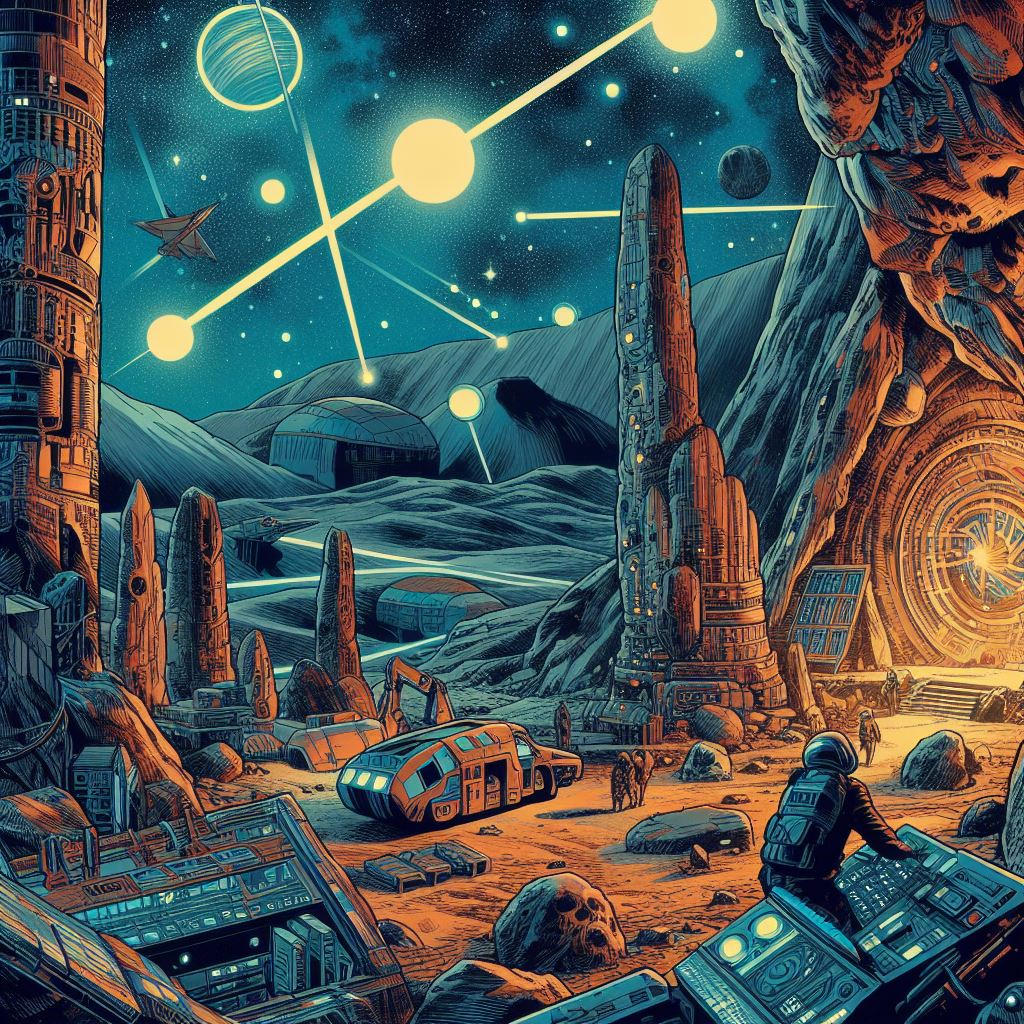
\includegraphics[width=\textwidth]{1}}};
        \node [ellipse callout, fill=white, draw, callout relative pointer={(.5,-.5)}] at (1,-1) {WOW!};
    \end{tikzpicture}
\end{minipage}%
\hfill
\begin{minipage}{0.48\textwidth}
    \begin{tikzpicture}
        \node (img) {\frame{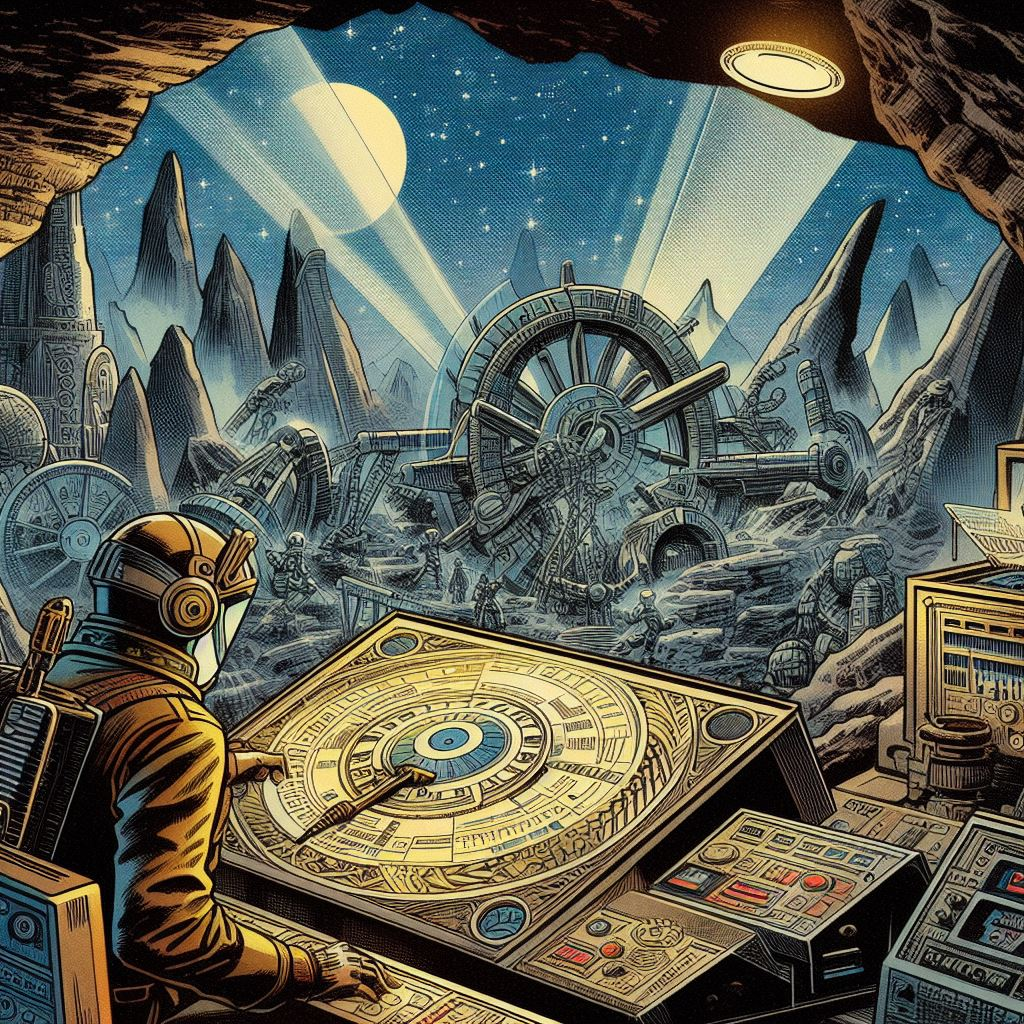
\includegraphics[width=\textwidth]{2}}};
        \node [text width=3.5cm,align=center,ellipse callout, fill=white, draw, callout relative pointer={(-1,-1)}] at (0,1) {\footnotesize THIS IS SIMPLY AMAZING! I STILL CANNOT BELIEVE IT};
    \end{tikzpicture}
\end{minipage}%
\vfill
\noindent\hspace{1pt}
\begin{minipage}{1\textwidth}
    \frame{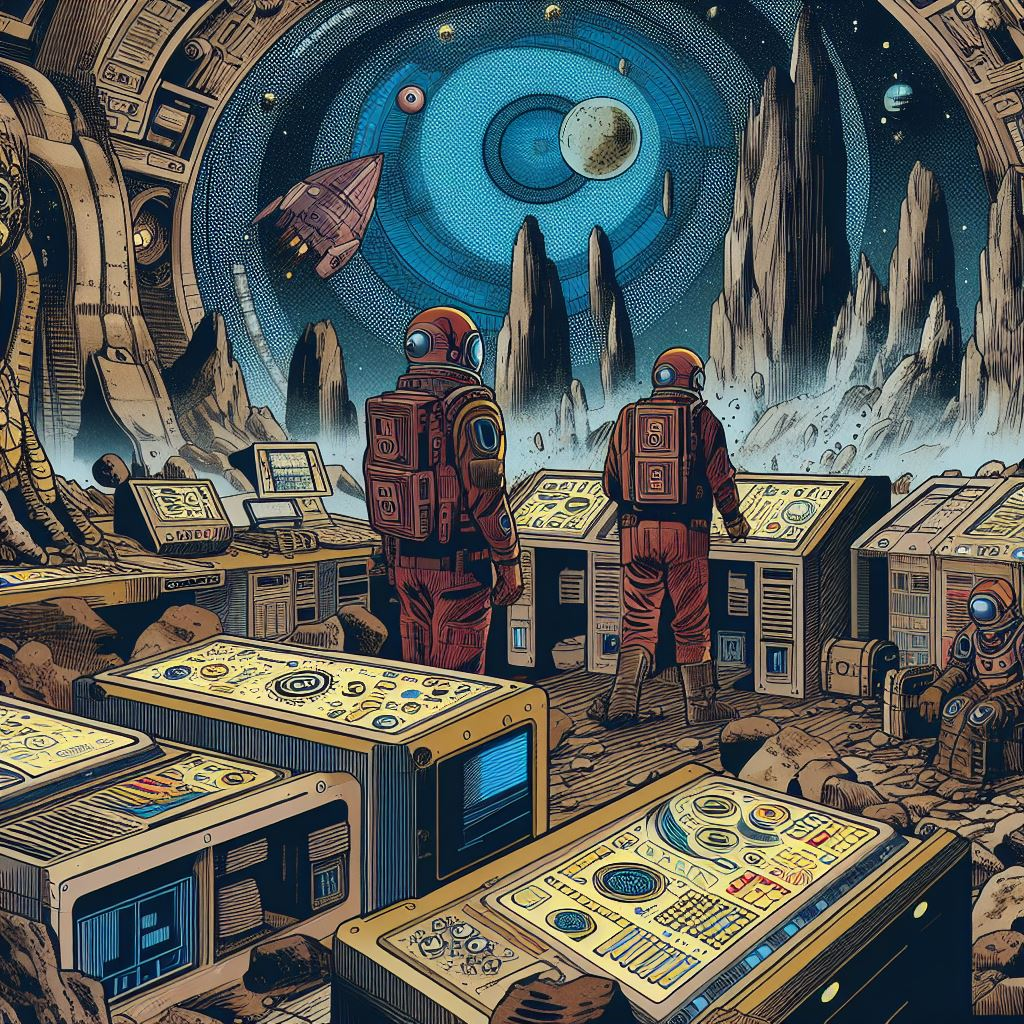
\includegraphics[width=\textwidth]{3}}
\end{minipage}%



\end{document}